% ============================================================
% PyQCD 学术报告：梯度流重整化下核子胶子 TMD-PDF
% 编译：xelatex 两遍；交付闸门：Overfull=0, Float too large=0,
% Missing character=0；页面：16:9 Beamer。
%
% frame_manifest（版式账本摘要）
% S1 标题；S2 结论；S3 研究对象/判据；S4 全链算法；S5 设置；
% S6 流；S7 RK3；S8 Clover/对偶；S9 staple/O；S10 ratio；
% S11 Z_R/混合；S12 Fourier/CS；S13 matching/SFTX；S14 外推；
% S15 工程；S16 验证；S17 归档图；S18 MyQCD 对照；S19 风险/下一步；
% A1--A3 源码与参考。每页主视觉为表格、公式、流程或图，来源行保留。
% ============================================================
\documentclass[UTF8,aspectratio=169,11pt]{ctexbeamer}

\usepackage{amsmath,amssymb}
\usepackage{graphicx}
\usepackage{booktabs}
\usepackage{tabularx}
\usepackage{array}
\usepackage{tikz}
\usetikzlibrary{arrows.meta,positioning,calc,fit,shapes.geometric}
\usepackage{listings}
\usepackage{xcolor}
\usepackage{microtype}
\usepackage{hyperref}

% 让源码索引中的路径在窄栏和页脚前可断行；不改变正文数学排版。
\def\UrlBreaks{\do\/\do-\do\_\do\.\do\:\do\;\do\?\do\&\do\=\do\%\do\#\do\@}
\Urlmuskip=0mu plus 1mu

\definecolor{primary}{HTML}{17365D}
\definecolor{accent}{HTML}{1F77B4}
\definecolor{evidence}{HTML}{1E8449}
\definecolor{warning}{HTML}{C55A11}
\definecolor{muted}{HTML}{5B6573}
\definecolor{panel}{HTML}{F4F7FA}
\definecolor{linegray}{HTML}{CBD5E1}
\definecolor{good}{HTML}{EAF5EE}
\definecolor{warnbg}{HTML}{FFF4E8}
\definecolor{reference}{HTML}{7D3C98}

\setmonofont{DejaVu Sans Mono}
\setbeamersize{text margin left=0.55cm,text margin right=0.55cm}
\setlength{\columnsep}{0.22cm}
\setlength{\tabcolsep}{3pt}
\renewcommand{\arraystretch}{0.92}
\setlength{\emergencystretch}{3em}
\setlength{\parskip}{0pt}
\setbeamertemplate{navigation symbols}{}
\setbeamertemplate{blocks}[rounded][shadow=false]
\setbeamercolor{normal text}{fg=black!86,bg=white}
\setbeamercolor{structure}{fg=primary}
\setbeamercolor{frametitle}{fg=primary,bg=white}
\setbeamercolor{block title}{fg=primary,bg=panel}
\setbeamercolor{block body}{fg=black!86,bg=panel}
\setbeamerfont{frametitle}{size=\large,series=\bfseries}
\setbeamerfont{normal text}{size=\normalsize}
\setbeamertemplate{frametitle}{%
  \vskip0.12cm\insertframetitle\par\vskip0.08cm}
\setbeamertemplate{footline}{%
  \hbox{\begin{beamercolorbox}[wd=\paperwidth,ht=2.3ex,dp=0.9ex,
    leftskip=0.55cm,rightskip=0.55cm]{author in head/foot}%
    \scriptsize\color{muted}PyQCD\hfill
    \insertshorttitle\hfill\insertframenumber/\inserttotalframenumber
  \end{beamercolorbox}}}

\newcommand{\source}[1]{%
  \par\vspace{0.02em}\begingroup\fontsize{6}{6.8}\selectfont\raggedright\sloppy
  \setlength{\emergencystretch}{3em}\rightskip=0pt plus 2em
  \color{muted}来源：#1\par\endgroup}
\newcommand{\verified}{\textcolor{evidence}{确证}}
\newcommand{\inferred}{\textcolor{accent}{推断}}
\newcommand{\unverified}{\textcolor{warning}{未验证}}
\newcommand{\refstate}{\textcolor{reference}{辅助参考}}
\newcommand{\Tr}{\operatorname{Tr}}
\newcommand{\dd}{\mathrm{d}}
\newcommand{\R}{\mathbb{R}}
\newcolumntype{Y}{>{\raggedright\arraybackslash}X}

\tikzset{
  flow/.style={draw=accent,fill=accent!8,rounded corners=2pt,align=center,
    minimum height=0.67cm,text width=2.08cm,font=\scriptsize},
  state/.style={draw=primary,fill=primary!7,rounded corners=2pt,align=center,
    minimum height=0.67cm,text width=2.45cm,font=\small},
  decision/.style={draw=warning,fill=warning!10,diamond,aspect=2.0,align=center,
    inner sep=1.5pt,font=\scriptsize},
  arrow/.style={-{Latex[length=2mm]},draw=primary,semithick},
  relation/.style={-{Latex[length=1.7mm]},draw=muted,thin,dashed},
  labelstyle/.style={font=\scriptsize,inner sep=1.5pt,fill=white,text=muted}
}

\lstset{
  language=Python,
  basicstyle=\ttfamily\scriptsize,
  backgroundcolor=\color{panel},frame=single,
  breaklines=true,breakatwhitespace=false,keepspaces=true,
  columns=flexible,firstnumber=auto,
  keywordstyle=\color{primary}\bfseries,
  commentstyle=\color{evidence!70!black},
  stringstyle=\color{accent},
  numbers=left,numberstyle=\tiny\color{muted}
}
\hypersetup{colorlinks=true,linkcolor=accent,urlcolor=accent}

\title[PyQCD 梯度流胶子 TMD-PDF]{PyQCD：梯度流重整化下\\核子胶子 TMD-PDF}
\subtitle{格点 QCD 算法实现、物理映射与验证边界}
\author[代码—物理分析]{PyQCD 代码—物理分析}
\institute{格点 QCD：从规范组态到可检验的胶子 TMD 链}
\date{2026 年 8 月 28 日}

\begin{document}

\begin{frame}[plain]
  \titlepage
\end{frame}

\begin{frame}[t]{核心判断：代码链已闭合，精密物理闭环仍需分层验收}
  \begin{columns}[T,totalwidth=\textwidth]
    \begin{column}{0.30\textwidth}
      \begin{block}{代码层：确证}
        已有 Wilson flow RK3、Clover/对偶场强、staple Wilson 线、
        TMD 组合、断连 ratio、\(Z_R\)/混合、傅里叶、NLO 核与联合外推入口。

        \vspace{0.2em}
        当前会话实测：\textbf{41 passed, 0 failed}。
      \end{block}
    \end{column}
    \begin{column}{0.30\textwidth}
      \begin{block}{算法层：可运行}
        随机 \(SU(3)\) demo 实测
        \(E:0.1908\to0.1904\)，输出
        \(O(z,b_\perp)\)、自重整化比值、准 TMD、CS 核与 SFTX 系数。

        归档 test9 有 \(N_{\rm conf}=10\)、\(13\times5\) OPE/拟合图表。
      \end{block}
    \end{column}
    \begin{column}{0.30\textwidth}
      \begin{block}{物理层：未验证边界}
        \unverified\ 归档原始数据不在当前工作树；
        完整 TMD 软因子、rapidity subtraction、staple 长度外推和连续极限物理结果，
        不能由单元测试或已有图片替代。
      \end{block}
    \end{column}
  \end{columns}
  \vfill
  \begin{beamercolorbox}[wd=0.98\textwidth,sep=0.65em,rounded=true]{block body}
    \textbf{本报告的结论边界：}PyQCD 已提供一条可复现、可测试的算法骨架；
    “实现了计算链”不等于“已经得到统计可靠的物理 TMD-PDF”。
  \end{beamercolorbox}
  \source{代码：\nolinkurl{pyqcd/renorm/}、\nolinkurl{pyqcd/operator/}、\nolinkurl{pyqcd/analysis/}；实测：\nolinkurl{examples/pyqcd/conftest.py}。}
\end{frame}

\begin{frame}[t]{研究对象与验收标准：TMD 比准 PDF 多一个横向坐标尺度}
  \begin{columns}[T,totalwidth=\textwidth]
    \begin{column}{0.46\textwidth}
      \begin{block}{物理对象}
        \begin{align*}
          H_g(z,\boldsymbol b_\perp;P_z,\tau,\ell)
          &\longrightarrow
          x\,\widetilde g(x,\boldsymbol b_\perp;P_z),\\[-0.2em]
          x\,\widetilde g
          &\sim \mathcal N_g\int\frac{\dd z}{2\pi}\\[-0.2em]
          &\quad e^{\,ixzP_z}H_g(z,\boldsymbol b_\perp).
        \end{align*}
        \(z\) 是纵向 Fourier 变量，\(\boldsymbol b_\perp\) 是横向坐标空间变量，
        \(\mu\) 是 UV 标度，\(\zeta\) 是快度标度；\(\tau\) 与 \(\ell\) 是额外的流/几何控制量。
      \end{block}
    \end{column}
    \begin{column}{0.48\textwidth}
      \small
      \begin{tabularx}{\linewidth}{@{}lYl@{}}
        \toprule
        验收层 & 必须回答的问题 & 当前状态\\
        \midrule
        规范结构 & 两个场强插入是否由同一几何的 Wilson 线连接？ & \verified\\
        流时间 & \(a^2\ll\tau\) 且不吞没物理分离的窗口是否存在？ & \unverified\\
        外态 & 核子 2pt/断连插入是否给出稳定平台？ & 部分\\
        重整化 & \(Z_R\)、软因子、匹配与快度演化是否同一方案？ & 部分\\
        极限 & \(b_\perp\to0\)、\(P_z\to\infty\)、\(a\to0\) 是否稳定？ & \unverified\\
        统计 & 协方差、样本数与误差带是否足够？ & 风险\\
        \bottomrule
      \end{tabularx}
    \end{column}
  \end{columns}
  \vfill
  \textcolor{warning}{报告只把直接代码/测试支持的内容标为确证；其余写成推断或未验证。}
  \source{参考：MyQCD TMD 软函数章节（见附录 C）；实现：\nolinkurl{pyqcd/renorm/_tmd.py}。}
\end{frame}

\begin{frame}[t]{端到端算法：每一步的输出都是下一步的输入}
  \centering
  \small
  \begin{tabular}{@{}l@{}}
    \textbf{输入：}\(U_\mu(x)\in SU(3)\)，ILDG 组态、蒸馏本征模/传播子与核子外态参数\\
    \quad \(U\) 读入并检查布局 \((N_t,N_z,N_y,N_x,4,3,3)\) 与链接幺正性\\
    \textbf{流化：}\(V_\tau\leftarrow\operatorname{WilsonFlow}_{\rm RK3}(U;\tau=3a^2,\varepsilon)\)\\
    \quad 检查 \(E(\tau)\) 相对初值下降，并监测 \(V_\tau V_\tau^\dagger-\mathbf1\)\\
    \textbf{算符：}\(F_{\mu\nu}\leftarrow\operatorname{Clover}(V_\tau),\quad
      \widetilde F\leftarrow\tfrac12\epsilon F,\quad W_{\rm st}\leftarrow\operatorname{staple}(z,b_\perp,\ell)\)\\
    \quad \(O=M^{tx;tx}+M^{ty;ty}-2M^{xy;xy}\to\operatorname{sum}_{\boldsymbol x}O(t,z,b_\perp)\)\\
    \textbf{外态统计：}\(C_3=C_2\,\mathrm{OPE}\to C_3-C_2\langle\mathrm{OPE}\rangle_0
      \to R(\mathrm dt,\mathrm d\tau,z,b_\perp)\to c_0\)\\
    \textbf{重整化：}\(c_0\to h_R\)（\(z=0\) 比值；或 \(Z_R+\) 混合方案）\\
    \textbf{分布重构：}\(h_R\xrightarrow{\cos/\sin\ Fourier}\widetilde g
      \xrightarrow{K,S_I,Z_{ij}}g\xrightarrow{a,P_z,m_\pi,L\;\mathrm{fit}}g_0\)\\
    \textbf{输出：}\(xg(x,b_\perp;\mu,\zeta)\)、误差带、诊断图、H5/JSON 与可追溯来源
  \end{tabular}
  \vfill
  \begin{tikzpicture}[node distance=0.28cm and 0.14cm]
    \node[flow] (u) {规范组态\\外态数据};
    \node[flow,right=of u] (f) {流化\\\(V_\tau\)};
    \node[flow,right=of f] (o) {Clover + staple\\\(O(z,b)\)};
    \node[flow,right=of o] (r) {ratio + 拟合\\\(c_0\)};
    \node[flow,right=of r] (p) {重整化 + Fourier\\\(\widetilde g\)};
    \node[flow,right=of p] (g) {匹配/外推\\\(g_0\)};
    \foreach \a/\b in {u/f,f/o,o/r,r/p,p/g}{\draw[arrow] (\a) -- (\b);}
  \end{tikzpicture}
  \source{编排：\nolinkurl{examples/pyqcd/test9_gluon_tmd_nucleon.py:84-301}；核心链：\nolinkurl{pyqcd/pipeline/_tmd9.py:1-224}。流程图为实现依赖关系示意。}
\end{frame}

\begin{frame}[t]{可复现设置：当前 test9 将格点、动量、流时间和横向网格显式化}
  \footnotesize
  \renewcommand{\arraystretch}{0.72}
  \begin{tabularx}{0.98\textwidth}{@{}p{0.13\textwidth}Yp{0.22\textwidth}Y@{}}
    \toprule
    项目 & 当前实现/实战设置 & 物理含义 & 来源\\
    \midrule
    系综 & \(24^3\times72\)，\(a=0.1053\,\mathrm{fm}\)，\(a^{-1}\simeq1.874\,\mathrm{GeV}\) & 空间有限体积与离散尺度 & \nolinkurl{pipeline/_config.py}\\
    组态 & \(6250,6450,\ldots,8050\)，共 10 个 & 统计样本；不是连续极限数据集 & 同上\\
    规范场布局 & \((N_t,N_z,N_y,N_x,4,3,3)\) & t,z,y,x 及 Lorentz/色矩阵轴 & \nolinkurl{_gluon_ope.py:63-76}\\
    动量 & \(\boldsymbol p=(p_z,p_y,p_x)\)，单位 \(2\pi/L\)；A 集合为 \(p_z=0,2,4\) & LaMET 大动量方向 & \nolinkurl{_tmd9.py:31-43}\\
    单位换算 & \(P_z^{\rm phys}=p_z\,2\pi/(N_l a)\) & 进入 Fourier/匹配的 GeV 动量 & \nolinkurl{_ensembles.py:38-40}\\
    TMD 网格 & \(z=0,\ldots,12\)，\(b_\perp=0,\ldots,4\) & 纵向分离与横向坐标空间采样 & \nolinkurl{test9.py:55-59}\\
    流 & \(\tau=3\)（格点单位），\(\varepsilon=0.05\)，约 60 步 & 对应约定 \(\tau=3a^2\)；需注意物理换算 & 同上\\
    精度/后端 & 默认 torch + complex64；可切换 numpy/complex128 & 速度、显存与舍入误差折中 & \nolinkurl{_torch_backend.py}\\
    \bottomrule
  \end{tabularx}
  \vspace{0.08em}
  \begin{beamercolorbox}[wd=0.98\textwidth,sep=0.18em,rounded=true]{block body}
    \scriptsize\textbf{量纲：}\(z,b_\perp\) 先是格点整数；进入准 PDF 转为 fm，再除以
    \(0.197\,\mathrm{GeV\,fm}\) 得 \(\mathrm{GeV}^{-1}\)。SFTX 的 \(\ln(\mu^2t)\) 要用 \(\mathrm{GeV}^{-2}\)。
  \end{beamercolorbox}
  \source{参数：\nolinkurl{pyqcd/pipeline/_config.py}；实战：\nolinkurl{examples/pyqcd/test9_gluon_tmd_nucleon.py}。}
\end{frame}

\begin{frame}[t]{梯度流：用规范作用量的下降方向抹平 UV，但流时间不是自由常数}
  \begin{columns}[T,totalwidth=\textwidth]
    \begin{column}{0.51\textwidth}
      \footnotesize
      \begin{block}{连续图像与格点生成元}
        \begin{align*}
          \partial_t B_\mu(t,x)&=D_\nu G_{\nu\mu}(t,x),
          &B_\mu(0,x)&=A_\mu(x),\\
          Z(V)&=P_{\rm ah}[\Omega_\mu V_\mu^\dagger],\\[-0.2em]
          P_{\rm ah}[M]&=\frac{M-M^\dagger}{2}
          -\frac{\Tr(M-M^\dagger)}{2N_c}\mathbf1.
        \end{align*}
        \(\Omega_\mu\) 是其余三个方向正反 6 个 staple 之和；
        \(Z\in\mathfrak{su}(3)\) 保持群流形更新。
      \end{block}
      \begin{block}{物理校验}
        流是规范场的扩散/耗散；测试窗口应有
        \(E(t)=\frac14G^2\downarrow\) 且 \(UU^\dagger\simeq\mathbf1\)。
        平滑半径量级为 \(\sqrt{8t}\)。
      \end{block}
    \end{column}
    \begin{column}{0.45\textwidth}
      \scriptsize
      \begin{tabularx}{0.94\linewidth}{@{}X@{}}
        \textbf{算法：Wilson flow}\\[0.2em]
        输入：\(U,\tau,\varepsilon\)\\
        \quad \(V\gets U\)，\(n=\mathrm{round}(\tau/\varepsilon)\)\\
        for \(k=1,\ldots,n\)：\\
        \quad \(Z_0\gets Z(V)\)；执行 RK3 单步\\
        \quad 每步重算 6-staple 生成元\\
        \quad 监测 \(E_k\) 与酉性\\
        end for\\
        输出：\(V_\tau\)，供同一流时间的算符使用\\[0.3em]
        \textbf{停止/警戒：}\\
        \quad \(E_k\) 不降：检查步长/输入链接\\
        \quad 酉性偏大：检查指数近似/投影\\
      \end{tabularx}
    \end{column}
  \end{columns}
  \source{实现：\nolinkurl{pyqcd/renorm/_gradient_flow.py}；参考：Lüscher 2010、MyQCD 梯度流章节。}
\end{frame}

\begin{frame}[t]{RK3 单步：三次生成元评估换取稳定的群流时间积分}
  \begin{columns}[T,totalwidth=\textwidth]
    \begin{column}{0.53\textwidth}
      \footnotesize
      \begin{tabular}{@{}l@{}}
        \textbf{输入：}\(V_t,\varepsilon\)\\
        \(W_0=V_t,\quad Z_0=Z(W_0)\)\\
        \(W_1=\exp\!\left(\frac{\varepsilon}{4}Z_0\right)W_0\)\\
        \(Z_1=Z(W_1)\)\\
        \(W_2=\exp\!\left(\frac{8\varepsilon}{9}Z_1
          -\frac{17\varepsilon}{36}Z_0\right)W_1\)\\
        \(Z_2=Z(W_2)\)\\
        \(V_{t+\varepsilon}=\exp\!\left(\frac{3\varepsilon}{4}Z_2
          -\frac{8\varepsilon}{9}Z_1+\frac{17\varepsilon}{36}Z_0\right)W_2\)\\
        \textbf{输出：}\(V_{t+\varepsilon}\)\\[0.3em]
        \textbf{局部误差：}\(O(\varepsilon^3)\)（实现约定）\\
      \end{tabular}
    \end{column}
    \begin{column}{0.43\textwidth}
      \begin{block}{实现落点}
        \lstinputlisting[basicstyle=\ttfamily\fontsize{6}{6.6}\selectfont,
          firstline=127,lastline=135,
          firstnumber=127]{/root/PyQCD/pyqcd/renorm/_gradient_flow.py}
      \end{block}
      \par\vspace{0.15em}
      \scriptsize\textbf{边界：}\(\texttt{su3\_exp}\) 是四阶级数加行列式归一；
      小步长测试通过，但不等同于精确矩阵指数。
    \end{column}
  \end{columns}
  \source{代码：\nolinkurl{pyqcd/renorm/_gradient_flow.py:45-59,125-135}；测试：\texttt{su3\_and\_dissipation}、\texttt{tau\_limit}。}
\end{frame}

\begin{frame}[t]{Clover 与对偶场强：局域场强离散化决定算符的紫外输入}
  \small
  \begin{columns}[T,totalwidth=\textwidth]
    \begin{column}{0.45\textwidth}
      \begin{block}{物理/数学定义}
        \begin{equation*}
          \begin{aligned}
            F_{\mu\nu}(x)&=-\frac{i}{8}\sum_{q=1}^{4}
            \left(P_q-P_q^\dagger\right),\\[-0.2em]
            \widetilde F_{\mu\nu}&=\frac12\epsilon_{\mu\nu\rho\sigma}F_{\rho\sigma}.
          \end{aligned}
        \end{equation*}
        四个 plaquette 位于 \((+\mu,+\nu),(-\mu,+\nu),(-\mu,-\nu),(+\mu,-\nu)\)，
        使局部离散化在平移/反射下对称。
      \end{block}
      \begin{block}{物理图像}
        \(F_{ti}\) 是色电场分量，\(F_{ij}\) 是色磁场分量；
        对偶张量把电/磁结构按 Levi--Civita 张量互换。
      \end{block}
    \end{column}
    \begin{column}{0.50\textwidth}
      \footnotesize
      \begin{tabular}{@{}p{1.8cm}p{5.1cm}@{}}
        \toprule
        代码状态 & 对应物理对象/检查\\
        \midrule
        \texttt{tensor4} & \(\frac12\epsilon_{\mu\nu\rho\sigma}\) 查表；避免手写符号错误。\\
        \texttt{Clover} & 四叶 Clover \(F_{\mu\nu}\)；返回格点矩阵。\\
        \texttt{dual\_F} & \(F\to\widetilde F\) 的张量 contraction。\\
        \texttt{LIME} & 大端 ILDG 数据；首链接酉性探针定位偏移。\\
        \texttt{direction}\\[-0.2em]\texttt{/FF} & 正/负方向、交叉 Lorentz 对与 FF 变体。\\
        \bottomrule
      \end{tabular}
      \vfill
      \begin{beamercolorbox}[wd=0.98\linewidth,sep=0.5em,rounded=true]{block body}
        \textbf{量纲边界：}plaquette/Clover 是无量纲格点对象；与连续 \(F_{\mu\nu}\) 比较时须明确 \(a\) 的幂次归一。
      \end{beamercolorbox}
    \end{column}
  \end{columns}
  \source{实现：\nolinkurl{pyqcd/operator/_gluon_ope.py}；测试：\nolinkurl{examples/pyqcd/conftest.py}。}
\end{frame}

\begin{frame}[t]{TMD 算符：横向分离必须由 staple Wilson 线承载规范协变性}
  \small
  \begin{columns}[T,totalwidth=\textwidth]
    \begin{column}{0.51\textwidth}
      \begin{align*}
        W_{\rm st}(z,b;L)&=U_z^\dagger((z{+}L)\hat z+b,b)\\[-0.2em]
        &\quad\times U_\perp((z{+}L)\hat z+b,(z{+}L)\hat z)\\[-0.2em]
        &\quad\times U_z((z{+}L)\hat z,z\hat z),\\
        M^{\mu\lambda;\nu\rho}&=\sum_{\boldsymbol x}
        \Tr\!\left[F^{\mu\lambda}(x+z\hat z+b)W_{\rm st}
        F^{\nu\rho}(x)W_{\rm st}^\dagger\right],\\
        O(z,b)&=M^{tx;tx}+M^{ty;ty}-2M^{xy;xy}.
      \end{align*}
      \begin{block}{为什么是这三个分量}
        权重 \((1,1,-2)\) 是面向核子前向矩阵元的横向投影组合；
        它把电/磁 Lorentz 结构组织成目标胶子 TMD 通道。其“乘性可重整”性质至少需要与相应微扰分析和 scheme 一起确认。
      \end{block}
    \end{column}
    \begin{column}{0.45\textwidth}
      \scriptsize
      \begin{tabularx}{0.94\linewidth}{@{}X@{}}
        \textbf{逐格点实现：}\\
        输入：流场 \(V_\tau,z,b_\perp,z\_dir,b\_dir,L\)\\
        \quad 计算 \(F_{01},F_{02},F_{12}\)\\
        \quad 每个 \((z,b)\) 构造三段 staple\\
        \quad 远端场强 roll 到 \(x+z\hat z+b\)\\
        \quad 色矩阵相乘并取 \(\Tr\)\\
        \quad 空间求和；时间轴可保留\\
        输出：\((n_z,n_b)\) 或 \((n_z,n_b,N_t)\)\\[0.3em]
        \textbf{几何警戒：}\\
        \quad \(L\) 默认取 \(z\)，未扫描 \(L\to\infty\)\\
        \quad \(b_\perp=0\) 才是共线退化检查\\
        \quad 不得把直线 OPE 误命名为 TMD\\
      \end{tabularx}
    \end{column}
  \end{columns}
  \source{实现：\nolinkurl{pyqcd/renorm/_tmd.py}；\(\pm z\) OPE：\nolinkurl{pyqcd/operator/_gluon_ope.py}。}
\end{frame}

\begin{frame}[t]{断连矩阵元提取：真空扣除与激发态模型把 OPE 接到核子外态}
  \begin{columns}[T,totalwidth=\textwidth]
    \begin{column}{0.50\textwidth}
      \begin{align*}
        C_3(\mathrm dt,\mathrm d\tau,z,b)&=C_2(\mathrm dt)\,\mathrm{OPE}(\mathrm d\tau,z,b),\\
        C_3^{\rm disc}&=C_3-C_2\langle\mathrm{OPE}\rangle_0,\\
        R&=\left\langle C_3^{\rm disc}/C_2\right\rangle_{t_i},\\
        R&=c_0+c_1e^{-\Delta E\,\mathrm d\tau}
        +c_1e^{-\Delta E(\mathrm dt-\mathrm d\tau)}.
      \end{align*}
      \begin{block}{极限校验}
        当插入点远离源/汇，指数激发态项应衰减，\(R\to c_0\)。
        这里的 \(c_0(z,b)\) 才是送入重整化链的裸矩阵元样本。
      \end{block}
    \end{column}
    \begin{column}{0.46\textwidth}
      \scriptsize
      \begin{tabularx}{\linewidth}{@{}X@{}}
        输入：\(C_2\) 与 flowed OPE \((n_z,n_b,N_t)\)\\
        \quad 构造相对时间数组\\
        \quad \(C_3\gets C_2\times\mathrm{OPE}\)（当前因子化实现）\\
        \quad delete-one jackknife 或 bootstrap\\
        \quad 真空扣除、时间源平均得 \(R\)\\
        \quad 逐 \((z,b)\) 用协方差 + svdcut 拟合\\
        \quad 奇异/小样本时保存 plateau 均值备份\\
        输出：\(c_0,c_1,\Delta E,\chi^2\) 及 ratio/fit 文件\\[0.3em]
        \textbf{统计警戒：}\(N_{\rm conf}=10\) 且点数较多时协方差易秩亏；
        归档有 \texttt{cond=inf}，不能只看 \(\chi^2\)。
      \end{tabularx}
    \end{column}
  \end{columns}
  \vfill
  \begin{beamercolorbox}[wd=0.98\textwidth,sep=0.25em,rounded=true]{block body}
    \scriptsize\textbf{实现钩子：}\nolinkurl{run_ratio2pt} 先做真空扣除 ratio，再逐 \((z,b_\perp)\)
    拟合；关键数组和重采样语句收录于附录。
  \end{beamercolorbox}
  \source{代码：\nolinkurl{pyqcd/analysis/_tmd_ratio.py:31-213}；模型：\nolinkurl{pyqcd/analysis/_disconnected.py:23-61}；归档：\nolinkurl{.../tmd_ratio/1_fit_report_P200.txt:1-14}。}
\end{frame}

\begin{frame}[t]{重整化分两条路径：test9 使用 z=0 比值，完整 Z\_R/混合模块另有入口}
  \begin{columns}[T,totalwidth=\textwidth]
    \begin{column}{0.48\textwidth}
      \footnotesize
      \begin{block}{当前 test9 端到端路径}
        \begin{equation*}
          h_R(z,b;P_z)=\frac{c_0(z,b;P_z)}{c_0(0,b;P_z)}.
        \end{equation*}
        这是逐样本 z=0 自归一，优点是简单且可直接进入准 TMD 变换；
        但它不自动等价于完整的 \(Z_R(z,a,\mu)\)、软函数或 rapidity subtraction。
      \end{block}
      \begin{block}{代码落点}
        \nolinkurl{pipeline/_tmd9.py:self_renormalize}；在
        \nolinkurl{run_tmd_pdf_chain} 中使用。
      \end{block}
    \end{column}
    \begin{column}{0.48\textwidth}
      \footnotesize
      \begin{block}{完整方案模块}
        \begin{align*}
          \ln Z_R={}&k\frac{z}{a\ln(a\Lambda)}\\[-0.2em]
          &+\frac12\ln\left(1+\frac{d}{\ln(a\Lambda)}\right)^2\\[-0.2em]
          &+\frac{5C_A}{3b_0}
          \ln\frac{\ln(1/a\Lambda)}{\ln(\mu/\Lambda)}\\[-0.2em]
          +(m_0+m_2a^2)z+f_1a+f_2a^2.
        \end{align*}
        \nolinkurl{fit_ZR} 支持多系综协方差拟合；
        \nolinkurl{fit_ZR_samples} 逐样本重拟合。
      \end{block}
      \begin{block}{混合方案}
        \(z<z_s\) 用 \(h_B(z,P_z)/h_B(z,0)\)；\(z\ge z_s\) 用
        \(h_B/Z_R\) 乘 \(\eta_s\)，再以
        \(l_1\lambda^{-a_1}e^{-\lambda/\lambda_0}\) 外推。
      \end{block}
    \end{column}
  \end{columns}
  \source{入口：\nolinkurl{pyqcd/pipeline/_tmd9.py}；\(Z_R\)：\nolinkurl{pyqcd/renorm/_zr.py}；混合：\nolinkurl{pyqcd/renorm/_hybrid.py}。}
\end{frame}

\begin{frame}[t]{准 TMD、正弦交叉通道与 CS 核：Fourier 之前必须固定 convention}
  \scriptsize
  \begin{tabularx}{0.98\textwidth}{@{}p{0.13\textwidth}Yp{0.16\textwidth}Y@{}}
    \toprule
    算法对象 & 离散物理关系 & 输入/输出 & 当前边界\\
    \midrule
    准 TMD & \(x\widetilde g\propto\int_0^{z_{\max}}\!\dd z\,\cos(xzP_z)h_R(z,b)\)；\(\mathcal N=(P_z/P_t)^2\) & \(h_R(z,b)\to(n_x,n_b)\) & test9 直接有限区间余弦积分\\
    共线 sin & \(\widetilde g(x)\propto(2P_z/x)\int\dd z\,h(z)\sin(xP_zz)\) & \(h(z)\to(n_x)\) & \(x=0\) 保护置零；用于 \(b\to0\) 交叉校验\\
    CS 核 & \(K(b)=\bigl[\ln h_1-\ln h_2\bigr]/\ln(P_{z1}/P_{z2})\)，\(h_i=h_R(z_{\rm ref},b;P_{zi})\) & 两动量矩阵元 \(\to K(b)\) & 默认 \(z_{\rm ref}=1\)，并 clip \([-3,3]\)\\
    大 \(\lambda\) & \(h_R(\lambda)\sim l_1\lambda^{-a_1}e^{-\lambda/\lambda_0}\) & 长距尾拟合 & \texttt{\_hybrid.py} 支持；test9 主路径未调用\\
    \bottomrule
  \end{tabularx}
  \vfill
  \begin{beamercolorbox}[wd=0.98\textwidth,sep=0.55em,rounded=true]{block body}
    \textbf{极限检查：}\(b_\perp\to0\) 时 TMD 应与相应共线 convention 可比；
    \(P_z\) 增大时 LaMET 幂修正应减小。代码通过有限性/形状测试，尚未由当前工作树中的多组态原始数据建立连续极限曲线。
  \end{beamercolorbox}
  \source{实现：\nolinkurl{pyqcd/renorm/_tmdextract.py:30-158}、\nolinkurl{pyqcd/renorm/_hybrid.py:59-153}；辅助参考的 CS 比值：\nolinkurl{/root/MyQCD/refer/papers/TMD_Soft_Function_LaMET_latex/chapters/section02.tex:67-81}。}
\end{frame}

\begin{frame}[t]{NLO 匹配与 SFTX：微扰核、软因子和快度演化不能混为一个系数}
  \footnotesize
  \begin{columns}[T,totalwidth=\textwidth]
    \begin{column}{0.49\textwidth}
      \begin{block}{TMD 匹配结构}
        \begin{align*}
          x\widetilde g(x,b)&=\int\frac{\dd y}{|y|}
          C^{\rm hybrid}\!\left(\frac{x}{y},\lambda_s,\frac{\mu}{yP_z}\right)
          \frac{y g(y,b)}{\sqrt{S_I(b,\mu)}}
          e^{\frac12\ln(\zeta_z/\zeta)K(b)},\\
          C^{\rm hybrid}(\xi)&=\delta(1-\xi)
          +\frac{\alpha_s C_A}{2\pi}g(\xi,y).
        \end{align*}
        \(g\) 按 \(\xi<0\)、\(0<\xi<1\)、\(\xi>1\) 分区，
        并含共同的 \(g_0\) 正弦积分截断项。
      \end{block}
      \begin{block}{离散实现}
        \(Z_{ij}=\delta_{ij}+\frac{\alpha_s C_A}{2\pi}M_{ij}\)，
        通过矩阵求逆作用在每个 \(b_\perp\) 通道。
      \end{block}
    \end{column}
    \begin{column}{0.47\textwidth}
      \scriptsize
      \begin{tabularx}{\linewidth}{@{}p{1.25cm}X@{}}
        \toprule
        层次 & 代码职责/物理含义\\
        \midrule
        核函数 & 单圈 \(g_0\)--\(g_3\)，含 \(\operatorname{Si}\)、\(\lambda_s\)。\\
        TMD 混合 & 构造 \(Z_{ij}\)，加入 \(K(b)\)、\(\sqrt{S_I}\)。\\
        ratio 核 & ratio 方案胶子核，与一般 TMD 核分开。\\
        SFTX & \(O_{\overline{\rm MS}}=[1+\alpha_s c/(4\pi)]O_{\rm flow}\)。\\
        soft & 当前是输入比值的 \(R/R(0)\) 归一框架。\\
        \bottomrule
      \end{tabularx}
      \vfill
      \begin{beamercolorbox}[wd=0.98\linewidth,sep=0.28em,rounded=true]{block body}
        \scriptsize\unverified\ test9 主链尚未显式计算矩形 Wilson loop
        \(Z_E(2\ell,b)\)；soft/rapidity 闭合待补。
      \end{beamercolorbox}
    \end{column}
  \end{columns}
  \source{匹配：\nolinkurl{pyqcd/renorm/_matching.py}、\nolinkurl{pyqcd/renorm/_tmdextract.py}；SFTX 同文件；软因子参考见附录 C。}
\end{frame}

\begin{frame}[t]{连续极限入口：把离散、有限动量、手征和体积效应写进同一设计矩阵}
  \begin{columns}[T,totalwidth=\textwidth]
    \begin{column}{0.48\textwidth}
      \begin{equation*}
        \begin{aligned}
          f(x;a,P_z,m_\pi,L)={}&xg_0(x)+f_xa^2+l_xa^4\\
          &+h_xa^2P_z^2+\frac{d_x}{P_z^2}+\frac{b_x}{P_z}\\
          &+k_x(m_\pi^2-m_{\pi,\rm phy}^2)+c_xe^{-La m_\pi}.
        \end{aligned}
      \end{equation*}
      \begin{block}{物理分解}
        \(a^2,a^4\)：离散误差；\(a^2P_z^2\)：混合离散—动量项；
        \(1/P_z,1/P_z^2\)：LaMET 幂修正；\(m_\pi^2\)：手征偏离；
        指数项：有限体积。
      \end{block}
    \end{column}
    \begin{column}{0.48\textwidth}
      \footnotesize
      \begin{tabular}{@{}l@{}}
        输入：多系综 \((x,h_R,a,P_z,m_\pi,L)\) 与 boot 样本\\
        \quad 逐 \(x\) 构造 8 项设计行并做 Cholesky 白化\\
        \quad 非正定时回退单位权重并记录\\
        \quad 放开 \((xg_0,f_x,d_x,k_x)\)，逐样本 \(\mathrm{lstsq}\)\\
        输出：物理点估计、std、\(\chi^2\) 诊断\\[0.25em]
        \textbf{退化检查：}\\
        \quad 数据点少于自由参数：输出 NaN，不伪造极限\\
        \quad 协方差非正定：记录回退，而非静默改权重\\
      \end{tabular}
    \end{column}
  \end{columns}
  \vspace{0.08em}
  \begin{beamercolorbox}[wd=0.98\textwidth,sep=0.28em,rounded=true]{block body}
    \scriptsize\unverified\ 该入口有合成数据测试；当前 test9 仅在单一 \(L24\times72\) 系综上生成 PDF，
    不能称为已完成的 \(a/P_z/m_\pi/L\) 联合连续极限。
  \end{beamercolorbox}
  \source{模型：\nolinkurl{pyqcd/renorm/_extrapolate.py}；测试：\texttt{test\_extrapolate\_boot\_fit}；编排：\nolinkurl{examples/pyqcd/test9_gluon_tmd_nucleon.py}。}
\end{frame}

\begin{frame}[t]{工程实现：后端、IO、缓存和形状守卫把物理算法变成可回放管线}
  \footnotesize
  \renewcommand{\arraystretch}{0.82}
  \begin{tabularx}{0.98\textwidth}{@{}p{0.13\textwidth}Yp{0.22\textwidth}Y@{}}
    \toprule
    工程对象 & 实现方式 & 对物理链的作用 & 风险/守卫\\
    \midrule
    后端 & numpy/cupy/torch 统一适配；torch 可 CPU/CUDA & 同一张量公式可迁移到 GPU & dtype/设备混用会隐式升精度\\
    精度 & complex64/complex128 全局切换 & 显存—舍入误差可控 & 匹配矩阵和指数尾对精度敏感\\
    H5 IO & \nolinkurl{save_tensor_h5/load_tensor_h5}，优先 H5、兼容旧 npy/npz & 逐组态中间量可缓存/续跑 & 大 flowed gauge 保存会引入 CPU 拷贝与 swap\\
    组态缓存 & \nolinkurl{flow_gauge_for_config} 可读缓存；TMD 默认可不保存流场 & 让昂贵的 flow 与 OPE 分离复用 & 缓存需绑定参数/精度/组态 ID\\
    形状契约 & OPE \((n_z,n_b,N_t)\)，ratio \((N_s,dt,dtau,n_z,n_b)\) & 防止时间/空间轴误置 & 轴序错误会伪造物理趋势\\
    数据守卫 & 原始文件存在性、形状、NaN、ETA/进度日志 & 长作业失败前暴露输入问题 & 当前真实集群路径不随仓库提供\\
    \bottomrule
  \end{tabularx}
  \vspace{0.1em}
  \begin{beamercolorbox}[wd=0.98\textwidth,sep=0.18em,rounded=true]{block body}
    \scriptsize
    \textbf{工程算法：}输入数据 \(\to\) 后端转换 \(\to\) 单组态计算 \(\to\) H5 落盘
    \(\to\) 释放 GPU/GC \(\to\) 下一组态；分析/作图在 rank 0。
    \quad \textbf{最小原则：}物理对象、形状、单位和样本轴在模块边界记录。
  \end{beamercolorbox}
  \source{IO：\nolinkurl{pyqcd/tools/_io.py}；torch：\nolinkurl{pyqcd/tools/_torch_backend.py}；编排：\nolinkurl{pyqcd/pipeline/_tmd9.py}。}
\end{frame}

\begin{frame}[t]{验证矩阵：41/41 通过证明实现不变量，不替代真实系综的物理精度}
  \footnotesize
  \renewcommand{\arraystretch}{0.82}
  \begin{tabularx}{0.98\textwidth}{@{}p{0.13\textwidth}Yp{0.22\textwidth}Y@{}}
    \toprule
    验证域 & 代表测试/判据 & 本次结果 & 证据等级\\
    \midrule
    流 & \(SU(3)\) 酉性、\(E\) 下降、\texttt{tau\_limit} & PASS & 合成场/代码不变量\\
    算符 & TMD shape/finite、正负方向与 FF & PASS & 算法级确证\\
    重整化 & \(Z_R\)、hybrid ratio、boot 协方差、SFTX & PASS & 合成数据/有限性\\
    匹配 & 分区核、对称求和、TMD NLO、sin 准 PDF & PASS & 回归与边界保护\\
    统计 & ratio 拟合、plateau、CS、协方差回退 & PASS & 样本 + 形状契约\\
    工程 & torch/numpy、H5/环境、文件守卫、绘图 & PASS & 集成测试\\
    总体 & \nolinkurl{python examples/pyqcd/conftest.py} & \textbf{41 passed, 0 failed} & 本次会话实测\\
    \bottomrule
  \end{tabularx}
  \vspace{0.1em}
  \begin{beamercolorbox}[wd=0.98\textwidth,sep=0.18em,rounded=true]{block body}
    \scriptsize\textbf{推理边界：}“有限、形状正确、合成真值恢复”不能推出
    10 组态真实胶子 TMD 的信噪比、scheme 一致性或连续极限已收敛。
  \end{beamercolorbox}
  \source{实测：\texttt{python examples/pyqcd/conftest.py}，退出码 0；测试登记：\nolinkurl{examples/pyqcd/conftest.py}。}
\end{frame}

\begin{frame}[t]{归档图表：链路能落盘，但当前 \(c_0\) 统计应被视为风险信号}
  \begin{columns}[T,totalwidth=\textwidth]
    \begin{column}{0.48\textwidth}
      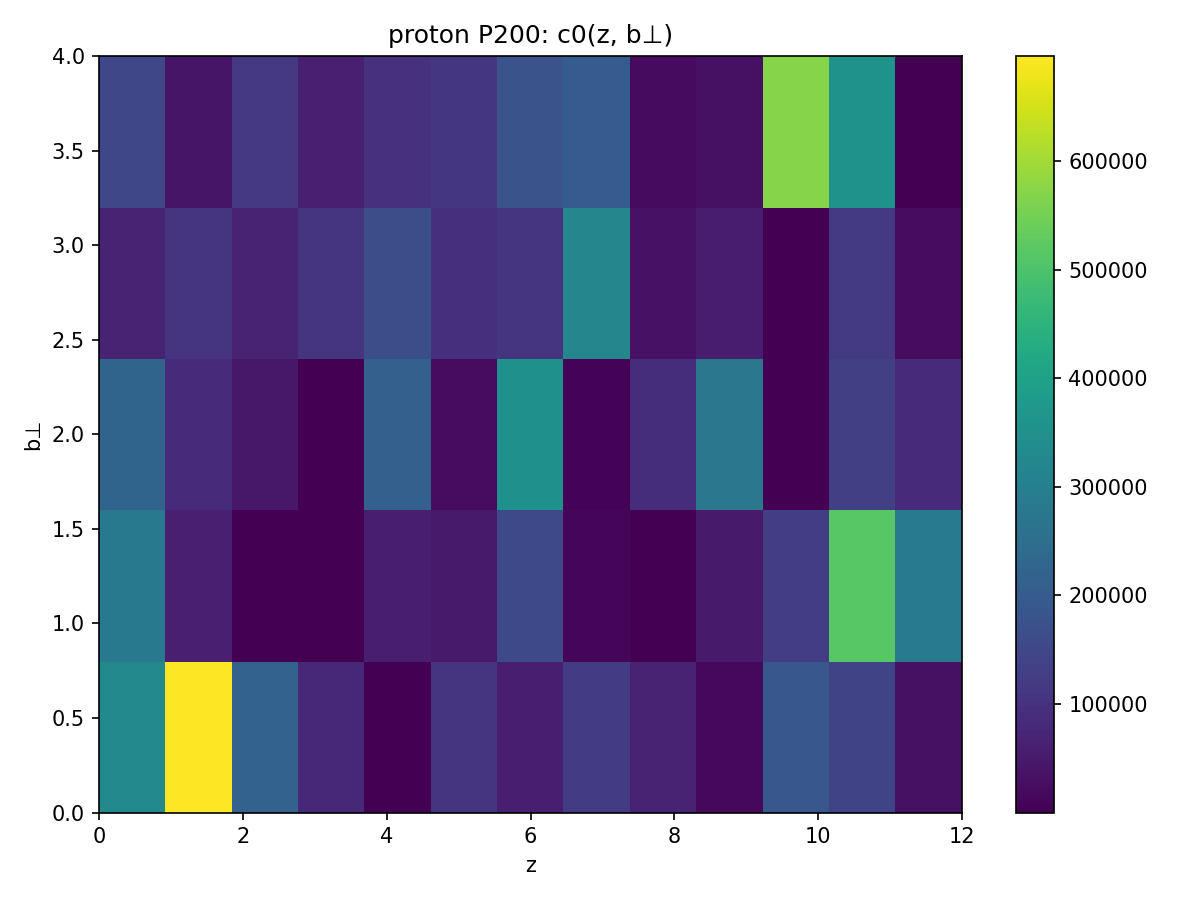
\includegraphics[width=\linewidth,height=0.28\textheight,keepaspectratio]{../examples/pyqcd/test9/analysis/tmd_ratio/c0_tmd_heatmap_proton_P200.png}
    \end{column}
    \begin{column}{0.48\textwidth}
      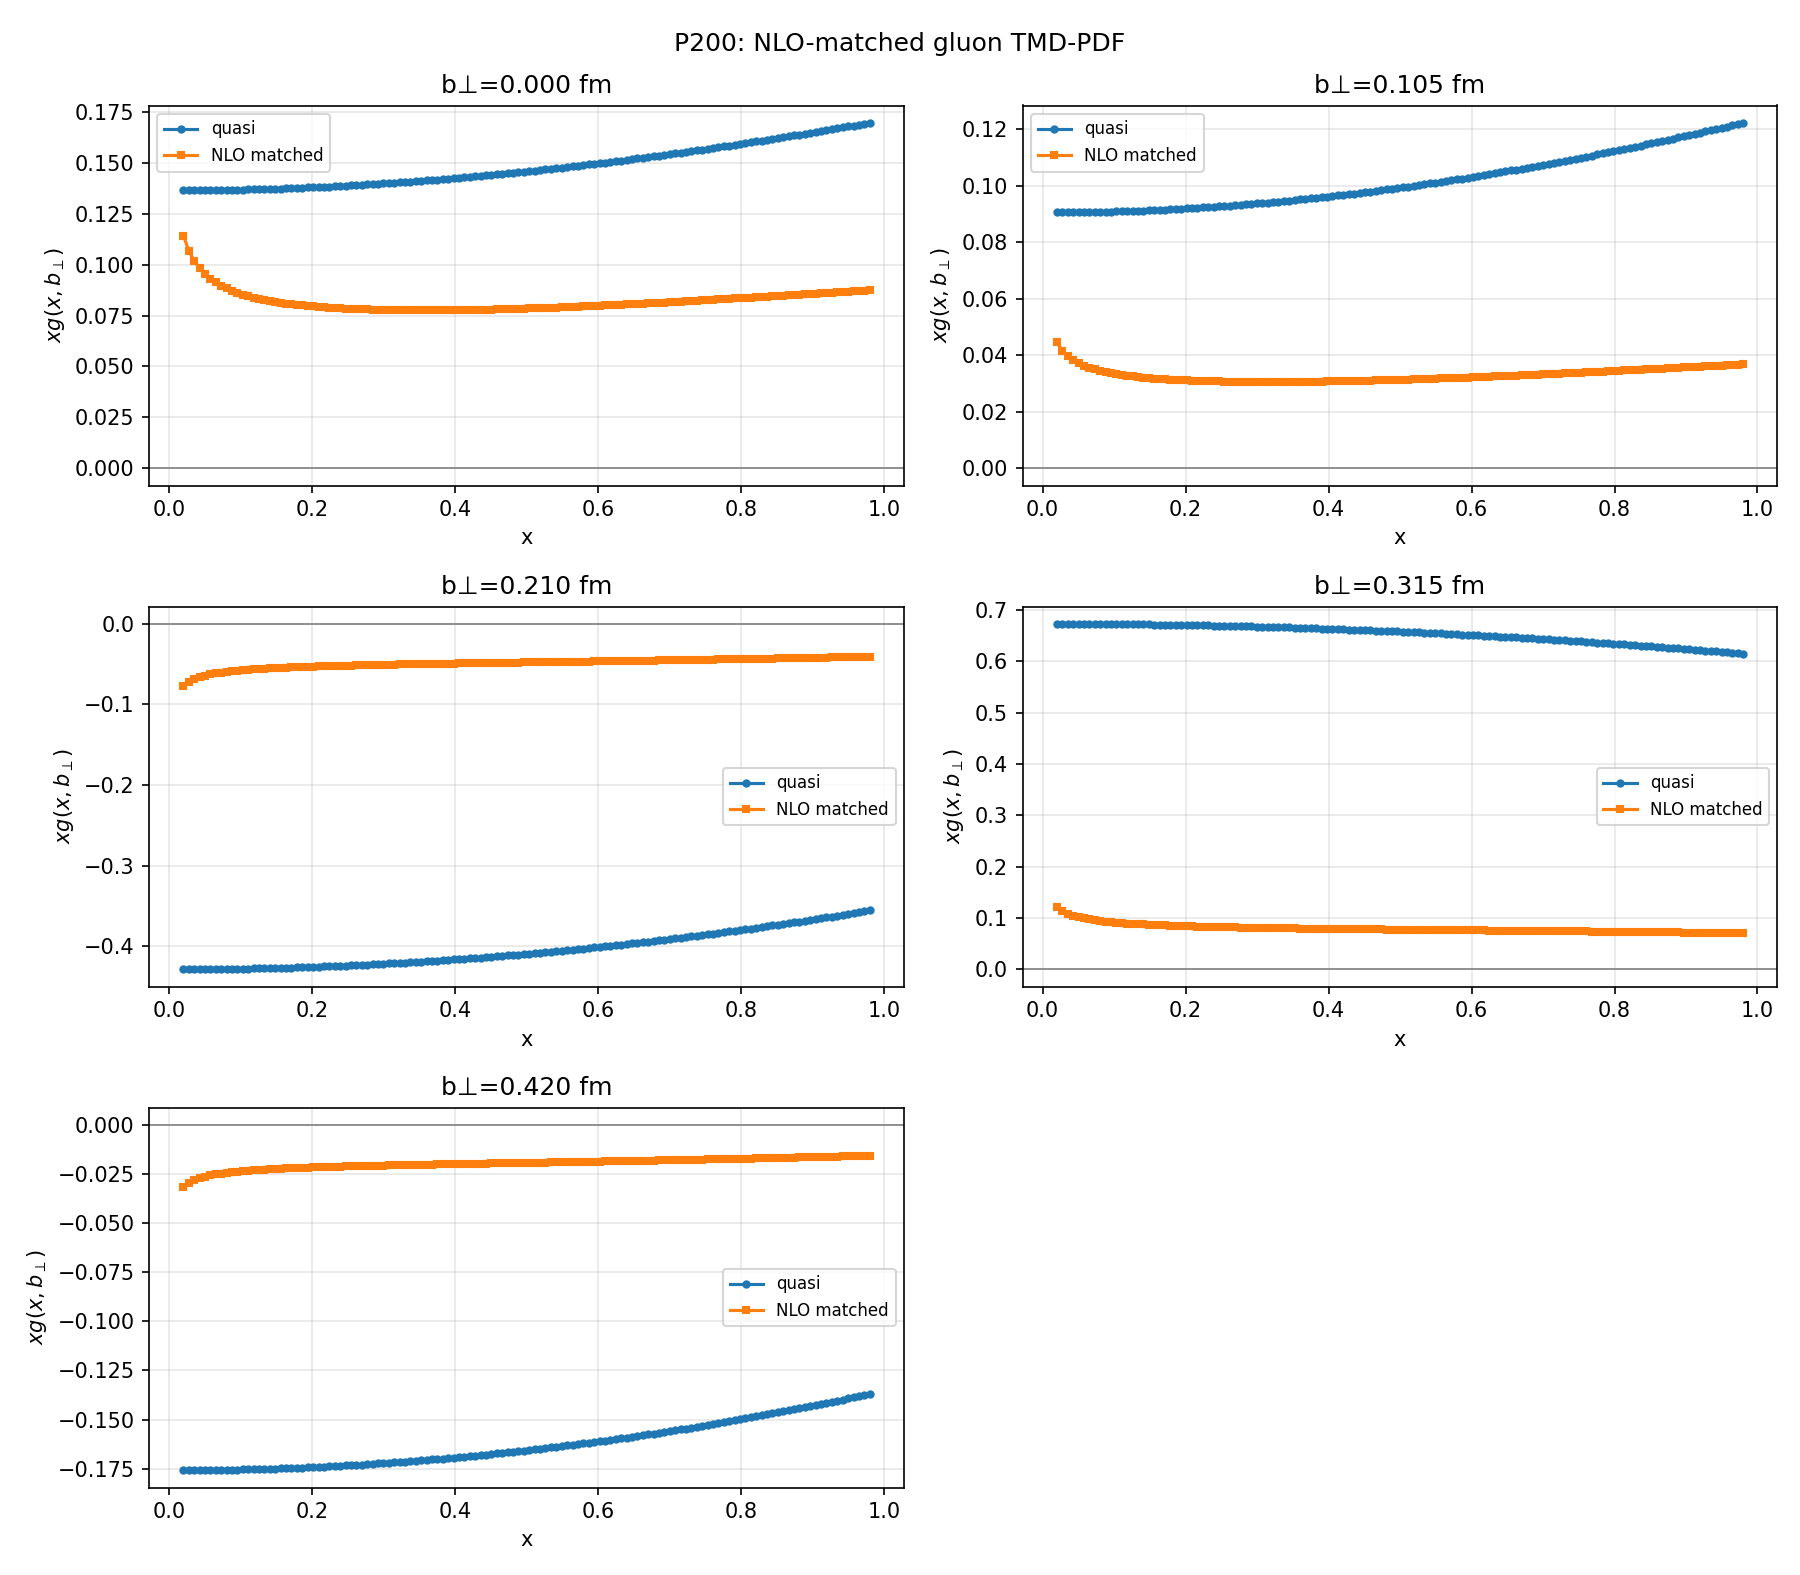
\includegraphics[width=\linewidth,height=0.28\textheight,keepaspectratio]{../examples/pyqcd/test9/analysis/tmd_ratio/matched_tmd_pdf.png}
    \end{column}
  \end{columns}
  \source{归档图：\nolinkurl{.../tmd_ratio/c0_tmd_heatmap_proton_P200.png}、\nolinkurl{.../tmd_ratio/matched_tmd_pdf.png}。}
  \scriptsize
  \begin{tabularx}{0.98\textwidth}{@{}p{0.30\textwidth}Y@{}}
    \toprule
    归档事实 & 解释边界\\
    \midrule
    P200 拟合报告标记 \(N_{\rm conf}=10\)、\(n_z\times n_b=13\times5\)、\(\mathrm dt\in[7,10]\)，且多处 \texttt{cond=inf}。 & 协方差秩亏；应优先增加统计或报告 plateau/boot 的敏感性。\\
    quasi/matched 图与 CS 图已生成。 & 证明分析与成图函数被调用，不单独证明 scheme 完备或曲线精确。\\
    \bottomrule
  \end{tabularx}
  \source{拟合文本：\nolinkurl{.../tmd_ratio/1_fit_report_P200.txt}；当前工作树无 test9 原始 H5/npy。}
\end{frame}

\begin{frame}[t]{MyQCD 辅助参考：用于物理几何与风险校验，不覆盖当前 PyQCD 状态}
  \footnotesize
  \renewcommand{\arraystretch}{0.82}
  \begin{tabularx}{0.98\textwidth}{@{}p{0.18\textwidth}Yp{0.23\textwidth}@{}}
    \toprule
    辅助参考 & 物理要点及 PyQCD 当前对应 & 状态差异\\
    \midrule
    梯度流 \nolinkurl{section02/03} & 流方程、平滑半径、流场重整化；对应 \nolinkurl{_gradient_flow.py} 的 RK3+\(E(t)\)。 & 已实现数值骨架\\
    TMD 软函数 & staple、矩形 Wilson loop \(Z_E(2\ell,b)\)、软因子比值；对应 staple/soft 接口。 & \(Z_E\) 未在 test9 主链显式实现\\
    CS 比值 & 双动量提取 \(K(b_\perp)\)，并标注 LO/幂修正边界；对应 CS 接口。 & 有 zref/clamp 保护；物理误差待测\\
    MyQCD 同名报告 & 较早阶段把 TMD 视作待新建模块；当前 PyQCD 已有 TMD、匹配和测试。 & 旧状态不能反向否定当前代码\\
    \bottomrule
  \end{tabularx}
  \vspace{0.1em}
  \begin{beamercolorbox}[wd=0.98\textwidth,sep=0.22em,rounded=true]{block body}
    \scriptsize\refstate\ \textbf{参考使用原则：}MyQCD 提供 staple/soft/CS 检查表；
    当前代码、参数和测试以 PyQCD 本地证据为准。
  \end{beamercolorbox}
  \source{辅助参考：MyQCD 的 TMD 软函数与梯度流章节；路径见附录 C。}
\end{frame}

\begin{frame}[t]{最大风险与下一步：先补物理闭环，再把图表升级为精密结果}
  \footnotesize
  \renewcommand{\arraystretch}{0.82}
  \begin{tabularx}{0.98\textwidth}{@{}p{0.08\textwidth}Yp{0.30\textwidth}Y@{}}
    \toprule
    顺序 & 可验收任务 & 通过判据 & 当前状态\\
    \midrule
    1 & 真实组态：保存 flowed gauge/OPE H5、env 与 A--E 日志 & 每组态 \(E\downarrow\)、酉性、shape、ratio/PDF 齐全 & 待补测\\
    2 & 扫描 staple 臂长 \(\ell\)，补同表示真空 Wilson loop/soft & \(\ell\) 平台、\(S_I\) 比值与动量无关 & 待实现/验证\\
    3 & 接入 \(Z_R\)+hybrid+\(\lambda\) 尾外推 & z 拼接连续；窗口/协方差敏感性可复现 & 模块已有，主链未闭合\\
    4 & \(b_\perp\to0\) 的 cos/sin 交叉与 representation 匹配 & 两通道 convention 相容；\(Z_{ij}\) 条件数可控 & 待补测\\
    5 & 多 \(a,P_z,m_\pi,L\) 系综联合外推 & 残差无结构、误差带覆盖、系统项可解释 & 入口已有，数据不足\\
    \bottomrule
  \end{tabularx}
  \vspace{0.1em}
  \begin{beamercolorbox}[wd=0.98\textwidth,sep=0.18em,rounded=true]{block body}
    \scriptsize\textbf{需决策：}非极化先行或加入 helicity；软因子表示及归一；
    多组态、多动量重跑的 GPU/存储额度。日程未给出，故不虚构截止日期。
  \end{beamercolorbox}
  \source{依据：模块缺口与 MyQCD 软函数/CS 对照；入口：\nolinkurl{examples/pyqcd/test9_gluon_tmd_nucleon.py}。}
\end{frame}

\appendix

\begin{frame}[t]{附录 A：RK3 与 TMD 组合的原文件直引}
  \begin{columns}[T,totalwidth=\textwidth]
    \begin{column}{0.47\textwidth}
      \begin{block}{Wilson flow 单步，原文件行 127--135}
        \lstinputlisting[firstline=127,lastline=135,
          firstnumber=127]{/root/PyQCD/pyqcd/renorm/_gradient_flow.py}
      \end{block}
    \end{column}
    \begin{column}{0.47\textwidth}
      \begin{block}{TMD 乘性组合，原文件行 158--161}
        \lstinputlisting[firstline=158,lastline=161,
          firstnumber=158]{/root/PyQCD/pyqcd/renorm/_tmd.py}
      \end{block}
      \begin{block}{对应物理式}
        \(O=M^{tx;tx}+M^{ty;ty}-2M^{xy;xy}\)。
        此处只显示实现语句；场强与 Wilson 线的构造见主体页及来源。
      \end{block}
    \end{column}
  \end{columns}
  \source{直引源文件：\nolinkurl{pyqcd/renorm/_gradient_flow.py}、\nolinkurl{pyqcd/renorm/_tmd.py}；代码片段未手抄。}
\end{frame}

\begin{frame}[t]{附录 B：匹配矩阵与 test9 参数的原文件证据}
  \footnotesize
  \begin{columns}[T,totalwidth=\textwidth]
    \begin{column}{0.52\textwidth}
      \begin{block}{TMD \(Z_{ij}\) 矩阵构造，原文件行 219--231}
        \lstinputlisting[basicstyle=\ttfamily\fontsize{5.8}{6.2}\selectfont,
          firstline=219,lastline=231,
          firstnumber=219]{/root/PyQCD/pyqcd/renorm/_tmdextract.py}
      \end{block}
    \end{column}
    \begin{column}{0.42\textwidth}
      \begin{block}{端到端参数}
        \scriptsize
        \renewcommand{\arraystretch}{0.78}
        \begin{tabular}{@{}ll@{}}
          \toprule
          参数 & 当前值\\
          \midrule
          \(z\) 网格 & 0--12\\
          \(b_\perp\) 网格 & 0--4\\
          \(\tau\) & 3（格点单位）\\
          \(\varepsilon\) & 0.05\\
          主动量 & P200；可用 P400 求 CS\\
          \(\mu\) & 2.0 GeV\\
          \(\lambda_s\) & 0.3 fm\\
          \bottomrule
        \end{tabular}
      \end{block}
      \begin{block}{注意}
        \scriptsize\texttt{x\_tmd} 是当前接口的匹配向量；
        与准/光锥输入的 convention 仍需明确。
      \end{block}
    \end{column}
  \end{columns}
  \source{直引：\nolinkurl{pyqcd/renorm/_tmdextract.py}；参数：\nolinkurl{examples/pyqcd/test9_gluon_tmd_nucleon.py}。}
\end{frame}

\begin{frame}[t]{附录 C：来源与验证索引}
  \scriptsize
  \renewcommand{\arraystretch}{0.78}
  \begin{tabularx}{0.98\textwidth}{@{}p{0.07\textwidth}Y@{}}
    \toprule
    ID & 可复查来源\\
    \midrule
    C1 & \nolinkurl{pyqcd/renorm/_gradient_flow.py:1-200}：Wilson flow、RK3、\(E(t)\)、\(t_0\)。\\
    C2 & \nolinkurl{pyqcd/operator/_gluon_ope.py:43-217}：Levi--Civita、Clover、对偶与 \(\pm z\) OPE。\\
    C3 & \nolinkurl{pyqcd/renorm/_tmd.py:52-305}：staple、\(O\) 组合、时间保留、比值与 CS 框架。\\
    C4 & \nolinkurl{pyqcd/analysis/_tmd_ratio.py:31-426}：断连 ratio、拟合、plateau、成图。\\
    C5 & \nolinkurl{pyqcd/renorm/_zr.py:25-342}、\nolinkurl{pyqcd/renorm/_hybrid.py:21-153}：\(Z_R\)/混合/样本环。\\
    C6 & \nolinkurl{pyqcd/renorm/_tmdextract.py:30-285}、\nolinkurl{pyqcd/renorm/_matching.py:20-172}：Fourier、CS、NLO/SFTX。\\
    C7 & \nolinkurl{pyqcd/renorm/_extrapolate.py:16-223}：连续极限设计矩阵与 boot WLS。\\
    C8 & \nolinkurl{pyqcd/pipeline/_tmd9.py:47-274}、\nolinkurl{examples/pyqcd/test9_gluon_tmd_nucleon.py:84-301}：端到端编排。\\
    T1 & 本次实测：\texttt{python examples/pyqcd/conftest.py}，退出码 0，\textbf{41 passed, 0 failed}。\\
    T2 & 本次实测：\texttt{python examples/pyqcd/tmd\_gradient\_flow\_demo.py}，随机 \(SU(3)\) 场 \(E:0.1908\to0.1904\)，全链输出有限。\\
    R1 & \nolinkurl{/root/MyQCD/refer/papers/TMD_Soft_Function_LaMET_latex/chapters/section02.tex:19-81}：staple/软因子/CS 参考。\\
    R2 & \nolinkurl{/root/MyQCD/refer/papers/Chiral_Symmetry_YM_Gradient_Flow_latex/chapters/section02.tex:24-42}：梯度流参考。\\
    \bottomrule
  \end{tabularx}
  \vspace{0.1em}
  \begin{beamercolorbox}[wd=0.98\textwidth,sep=0.35em,rounded=true]{block body}
    \textbf{最终判断：}当前交付物是“算法实现与物理边界报告”；精密 TMD-PDF 数值结论需在补齐软因子、真实数据和多尺度外推后另行报告。
  \end{beamercolorbox}
  \source{依据：PyQCD 源码、归档图表、本次测试及 MyQCD 辅助材料。}
\end{frame}

\end{document}
